% Figure: layered architecture of a QKDN (ITU-T Y.3800)
% (tikzpicture extracted from the paper figure, without the figure environment)
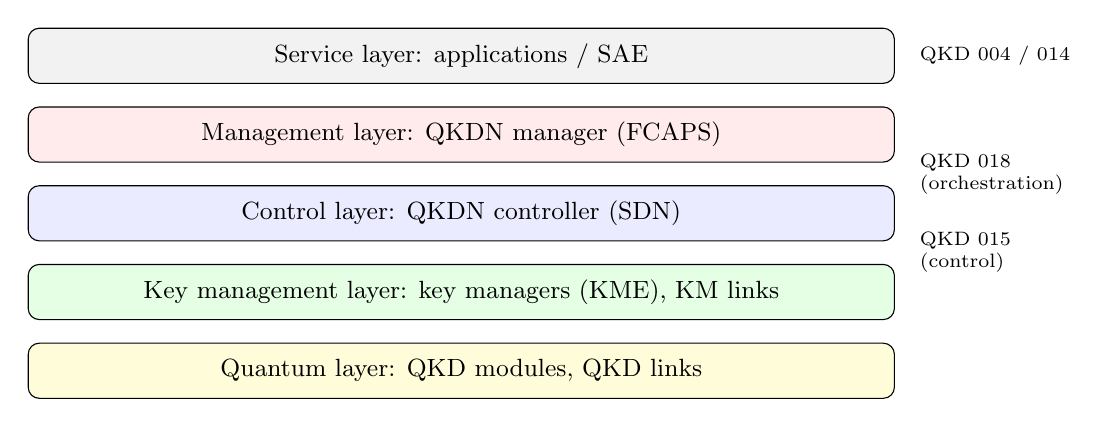
\begin{tikzpicture}[
  layer/.style={draw,rounded corners,minimum width=11cm,minimum height=7mm,
                align=center,font=\small},
  side/.style={font=\scriptsize,align=left,anchor=west}]
  \node[layer,fill=gray!10]   (srv) at (0,0)    {Service layer: applications / SAE};
  \node[layer,fill=red!8]     (mgm) at (0,-1.0) {Management layer: QKDN manager (FCAPS)};
  \node[layer,fill=blue!8]    (ctl) at (0,-2.0) {Control layer: QKDN controller (SDN)};
  \node[layer,fill=green!10]  (km)  at (0,-3.0) {Key management layer: key managers (KME), KM links};
  \node[layer,fill=yellow!15] (q)   at (0,-4.0) {Quantum layer: QKD modules, QKD links};
  \node[side] at (5.7,0)    {QKD 004 / 014};
  \node[side] at (5.7,-1.5) {QKD 018\\(orchestration)};
  \node[side] at (5.7,-2.5) {QKD 015\\(control)};
\end{tikzpicture}
